\section{Method Overview}
\label{sec:method}
\subsection{Problem Statement}
Given $M$ point sets with $I_m$ points $V_m=\{\pmb{v}_{mi}\}$ for the $m^{th}$ point set (Figure \ref{fig:teaser} (a) shows an example of input point sets.), we intend to simutaneously partition the point sets into $N$ objects and find the rigid transformations $\{\phi_{mn}(\pmb{x})=R_{mn}\pmb{x}+\pmb{t}_{mn}\}$ that transform each object model to its observed position in each input point set.  For partitioning, we output point-wise label vectors $\{\pmb y_m\}$ for each input point set to indicate its object partition. ( Figure~\ref{fig:teaser} (b) illustrates result label vectors by assigning same color to points with the same label. ) To establish our formulation, we first summarize the symbols that will be used in Table \ref{tab:symbol}.
\begin{table}[!hbp]
\centering
\begin{tabular}{c l}
\hline
Symbol & Meaning\\
\hline
$M$ & The number of input point sets.\\
$I_m$ & The number of points for $m^{th}$ point set.\\
$V$ & The input point sets.\\
$V_m$ & The $m^{th}$ input point set.\\
$\pmb v_{mi}$ & The $i^{th}$ point of $V_m$.\\
$\pmb f_{mi}$ & The point-wise feature vector of $\pmb v_{mi}$.\\
$z_{mi}$ & The latent parameter for $\pmb v_{mi}$.\\
& $z_{mi}=k$ means $v_{mi}$ is generated by $k^{th}$ Gaussian\\
$Z$ & $Z=\{z_{mi}|m=1...M,i=1...I_m\}$\\
$K_{all}$ & The total number of Gaussian models.\\
$K_n$   & The number of Gaussian for $n^{th}$ object. $\sum_n^N K_n = K_{all}$\\
$p_k$  & The weight of $k^{th}$ Gaussian. $\sum_k^{K_{all}}p_k=1$\\
$\pmb x_k$ & The centroid of $k^{th}$ Gaussian.\\
$\pmb {xv}_k$ & The centroid of $k^{th}$ Gaussian for point position.\\
$\pmb {xf}_k$ & The centroid of $k^{th}$ Gaussian for point feature.\\
$\Sigma_k$ & The covariance matrix of $k^{th}$ Gaussian.\\
$\sigma_k$ & $\Sigma_k=\sigma_k^2I$. ($I$ is identity matrix here.)\\
$\sigma v_k$ & Gaussian covariance parameter for point position\\
$\sigma f_k$ & Gaussian covariance parameter for point feature\\
$\phi_{mn}$ & Transformation from $n^{th}$ object to $m^{th}$ input set.\\
$R_{mn}$ & The rotation matrix for $\phi_{mn}$.\\
$\pmb t_{mn}$ & The translation vector for $\phi_{mn}$.
\end{tabular}
\caption{Table of Symbols Used in the Paper}
\label{tab:symbol}
\end{table}
\subsection{Basic Formulation}

To simutaneously model the joint registration and co-segmentation,  we come up with a generative model as follows:
\begin{equation}
\label{equ:model}
P(\pmb{v}_{mi})=\sum^{K_n}_{k=1}p_k\mathcal{N}(\pmb{v}_{mi}|\phi_{mn}(\pmb{x}_k),\Sigma_k)
\end{equation}
which treat the $i^{th}$ observed point $v_{mi}$ from the $m^{th}$ point set as a sample point generated by one of $N$ object models.
Each object model is represented by a group of $K_n$ gaussian models.\\
The model parameters are:
$$\Theta=\{\{p_k,\pmb x_k,\Sigma_k\}_{k=1}^{\sum{K_n}},\{\phi_{mn}\}_{m=1,n=1}^{MN}\}$$
The problem is how to estimate the parameters for the model to fit all the input point sets. The problem can be solved within the framework of expectation maximization. In particular, we bring in a latent parameter as:\\
$$Z=\{z_{mi}|m=1...M,n=1...I_m\}$$
such that $z_{mi}=k(k=1,2...,K_{all})$ assigns the observed point $v_{mi}$ to the $k^{th}$ component of Gaussian mixture model. We aim to maximize the expected complete-data log-likelihood:
\begin{equation}
\label{equ:obj0}
\mathcal{E}(\Theta|V,Z)=\mathbb{E}_Z[\ln P(V,Z;\Theta)|V]={\sum_ZP(Z|V,\Theta)\ln{P(V,Z;\Theta)}}
\end{equation}
Such formulation can be seen as an adaption of joint registration formulation in \cite{Evangelidis2014}, upon which we seperate Gaussian models into groups to express multiple objects. The latent parameter $Z$ that assigns observed points to Gaussian models can naturally indicate the object level segmentation.\\
By the asssumption that the input points are independent and identically distributed, we can rewrite the objective (\ref{equ:obj0}) into:
\begin{equation}
\label{equ:obj2}
\Theta=\arg\max\sum_{mik}\alpha_{mik}(\ln p_k + \ln P(\pmb v_{mi}|z_{mi}=k;\Theta))
\end{equation}
where $\alpha_{mik} = P( z_{mi} = k | \pmb v_{mi} ; \Theta )$\\
By bringing in equation \ref{equ:model} and ingnoring constant terms, we can rewrite the objective as:
\begin{equation}
\label{equ:obj3}
\Theta=\arg\max\sum_{mik}\alpha_{mik}(||\pmb v_{mi}-\phi_{mn}(\pmb x_k)||_{\Sigma_k}^2 + \ln |\Sigma_k| - 2\ln p_k)
\end{equation}
where the $|\cdot|$ denotes the determinant and $||x||_A^2=x^TA^{-1}x$. It is predefined that $x_k$ is one of the gaussian centroid used to represent $n^{th}$ object, which is why we apply transformation $\phi_{mn}$ on to the $x_k$. For the convenience of computation, we restrict the model to isotropic covariances, i.e.,$\Sigma_k=\sigma^2I$ and $I$ is the identity matrix.\\
Now, we can optimize this through iterating between estimating $\alpha_{mik}$ (Expectation-step) and maximizing $f(\Theta|V,Z)$ sequentially with respect to each parameters in $\Theta$ (Maximization-steps).
These steps are:\\
\textbf{E-step}:
this step estimates the posterior probability $\alpha_{mik}$ of $v_{mi}$ to be a point generated by the $k^{th}$ Gaussian model.\\
\begin{equation}
\label{equ:estep}
\alpha_{mik}=\frac{p_k\sigma_k^{-3}exp(-\frac{1}{2\sigma_k^2}||\pmb v_{mi}-\phi_{mn}(\pmb x_k)||^2)}{\sum_s^{K_{all}}p_s\sigma_s^{-3}exp(-\frac{1}{2\sigma_s^2}||\pmb v_{mi}-\phi_{mn}(\pmb x_s)||^2)}
\end{equation}
\textbf{M-step-a}:this step update the transformations $\phi_{mn}$ that maximize $f(\Theta)$, given instant values for $\alpha_{mik}$, $x_k$, $\sigma_k$. We only consider rigid transformations, making  $\phi_{mn}(x)=R_{mn}x+t_{mn}$. The maximizer $R_{mn}^*,t_{mn}^*$  of $f(\Theta)$ is the same with the minimizers of the following constrained optimization problems:\\
\begin{equation}
\left\{
\begin{array}{rcl}
\min_{R_{mn},t_{mn}}&      &||(W_{mn}-R_{mn}X_n-\pmb t_{mn}\mathbf{e}^T)\Lambda_{mn}||_F^2\\
s.t.&      &R_{mn}^TR_{mn}=I, |R_{mn}|=1\\
\end{array} \right.
\end{equation}
where $\Lambda_{mn}$ is $K_n \times K_n$ diagonal matrix with elements $\lambda_{mnk}=\frac{1}{\sigma_k}\sqrt{\sum_i^{I_{m}}\alpha_{mik}}$,$I_m$ is the number of point for the $m^{th}$ input point set, $X_n = [\pmb x_1, \pmb x_2,...., \pmb x_{K_n}]$ is the matrix stacked by the centroids of gaussian models that are predefined to represent the $n^{th}$ object. $\mathbf{e}^T$ is a vector of ones, $||\cdot||_F$ denotes the Frobenius norm, and $W_{mn}=[w_{m1},w_{m2},...,w_{mk},...,w_{mK_n}]$, in which $w_{mk}$ is a weighted point as:\\
\begin{equation}
w_{mk}=\frac{\sum_{i=1}^{I_m}\alpha_{mik} \pmb v_{mi}}{\sum_{i=1}^{I_m}\alpha_{mik}}
\end{equation}
This problem have a similar solution of in \cite{Evangelidis2014}. The only difference is that we are estimating the transformation from Gaussian models to the input point sets instead of the transformation from input point sets to Gaussian models, since there are multiple group of $\pmb x_k$ corresponding to multiple objects in our Gaussian models. The optimal can be given by:\\
\begin{equation}
\label{equ:updateR}
R_{mn}^*=U_{mn}C_{mn}V_{mn}^T
\end{equation}
\begin{equation}
\label{equ:updatet}
t_{mn}^*=\frac{1}{tr(\Lambda_{mn}^2)}(W_{mn}-R_{mn}X_n)\Lambda_{mn}^2\mathbf{e}
\end{equation}
where $[U_{mn},S,V_{mn}]=svd( W_{mn}\Lambda_{mn}P_{mn}\Lambda_{mn}X_{mn}^T )$ and $P_{mn}=I-\frac{\Lambda_{mn}\mathbf{e}(\Lambda_{mn}\mathbf{e})^T}{(\Lambda_{mn}\mathbf{e})^T\Lambda_{mn}\mathbf{e}}$,$I$ is identity matrix. $C_{mn}=diag(1,1,|U_{mn}||V_{mn}|)$.\\
\textbf{M-step-b}: this step we update the parameters related to the Gaussian mixture model and the indicating vector for object segmentation 
\begin{equation}
\label{equ:updatexk}
\pmb x_k^*=\frac{\sum_{m=1}^M\sum_{i=1}^{I_m}\alpha_{mik}(R_{mn}^{-1}v_{mi}-\pmb t_{mn})}{\sum_{m=1}^M\sum_{i=1}^{I_m}\alpha_{mik}}
\end{equation}
where $\pmb x_k$ is one of the Gaussian centroids that is predefined to represent $n^{th}$ object. 
\begin{equation}
\label{equ:updatesigma}
\sigma_k^{*2}=\frac{\sum_{m=1}^M\sum_{i=1}^{I_m}\alpha_{mik}||(v_{mi}-\pmb t_{mn}-R_{mn}^*\pmb x_k^*)||_2^2}{3\sum_{m=1}^M\sum_{i=1}^{I_m}\alpha_{mik}}
\end{equation}
\begin{equation}
\label{equ:updatepk}
p_k^*=\frac{\sum_{m,i}\alpha_{mik}}{M}
\end{equation}
\begin{equation}
\label{equ:updatey}
y_{m}(i)^*=\arg \max_n \sum_{k=K_{n-1}+1}^{K_n} \alpha_{mik} 
\end{equation}
where $y_{m}(i)$ is the $i^{th}$ entry of the indicate vector $y_m$.
\subsection{Bilateral Formulation}
When considering point-wise features, we can add bilateral terms into the generative model.
\begin{equation}
P(v_{mi},f_{mi})=\sum^{K_n}_{k=1}p_k\mathcal{N}(v_{mi}|\phi_{mn}(\pmb{xv}_k),\sigma v_k)\mathcal{N}(f_{mi}|\pmb{xf}_k,\sigma f_k)
\end{equation}
where $f_{mi}$ is the feature vector for point $v_{mi}$ and $xf_k$ is the feature vector for $k^{th}$ point in latent model. As shown in the formulation, there is no transformation applyed onto $xf_k$, which means that this formulation is only suitable to the features that is rotation and translation invariant. For example, the point color vector(for all the result in this paper we use RGB color as feature vector ) $[red_{mi},green_{mi},blue_{mi}]$ is a suitable feature for this formulation.In this formulation $N(v_{mi}|\phi_{mn}(xv_k),\sigma v_k)$ is the spatial term and $N(f_{mi}|xf_k,\sigma f_k)$ is the feature term.
For the bilateral formulation, iteration steps will be as follows:\\
\textbf{E-step}:in this step the calculation of posterior probability need to consider both the spatial term and the feature term.
\begin{equation}
\label{equ:bestep}
\alpha_{mik}=\frac{p_kP_v( \pmb v_{mi},\phi_{mn}(xv_k),\sigma v_k)P_f(f_{mi},xf_k,\sigma f_k)}{\sum_s^{K_{all}}p_sP_v( \pmb v_{mi},\phi_{mn}(xv_s),\sigma v_s)P_f(f_{mi},xf_k,\sigma f_s)}
\end{equation}
where $P_v(x,y,\sigma)=\sigma^{-3}exp(-\frac{1}{2\sigma^2}||x-y||^2)$ and $P_f(x,y,\sigma)=\sigma^{-D(\pmb x)}exp(-\frac{1}{2\sigma^2}||x-y||^2)$ and $D(\pmb x)$ means the dimension of the vector $\pmb x$.\\
\textbf{M-step-a:}for bilateral formulation, this step is the same with the basic formulation and the update can be done as (\ref{equ:updateR}) and (\ref{equ:updatet}).
\textbf{M-step-b}:for bilateral formulation, this step need not only update model centroids and variance for spatial term as (\ref{equ:updatexk}) and (\ref{equ:updatesigma}).
but also update the centroids and variance for feature term as in (\ref{equ:updatefk}) and (\ref{equ:updatefsigma})\\
\begin{equation}
\label{equ:updatefk}
xf_k^*=\frac{\sum_{m=1}^M\sum_{i=1}^{I_m}\alpha_{mik}f_{mi}}{\sum_{m=1}^M\sum_{i=1}^{I_m}\alpha_{mik}}
\end{equation}
\begin{equation}
\label{equ:updatefsigma}
\sigma f_k^{*2}=\frac{\sum_{m=1}^M\sum_{i=1}^{I_m}\alpha_{mik}||(f_{mi}-xf_k^*)||_2^2}{D(f)\sum_{m=1}^M\sum_{i=1}^{I_m}\alpha_{mik}}
\end{equation}
where $D(f)$ is the dimenssion of feature vectors.\\
The update of $p_k$ for bialateral formulation is the same as the basic formulation in (\ref{equ:updatepk}).
\subsection{Interaction Design}
\label{sec:imp:interact}
Unfortunately, there are a large number of parameters that can not be easily initialized in our formulation . In this subsection we first introduce our design of interaction, which is intuitive for users to input the semantic prior this way. We then explain how we can easily initlialize those parameters for our optimization based on the manual input.\\
As demonstrated in Figure~\ref{fig:interact}, we let user choose one of the point sets and placing and editing boxes in it to indicate the layout for this point set. From this, we can easily initialize the total number of objects $N$ and determine $\{K_n\}$ which is the numbers of Gaussian mixture models used to represent each object.
\begin{figure}[htb]
	\centering
	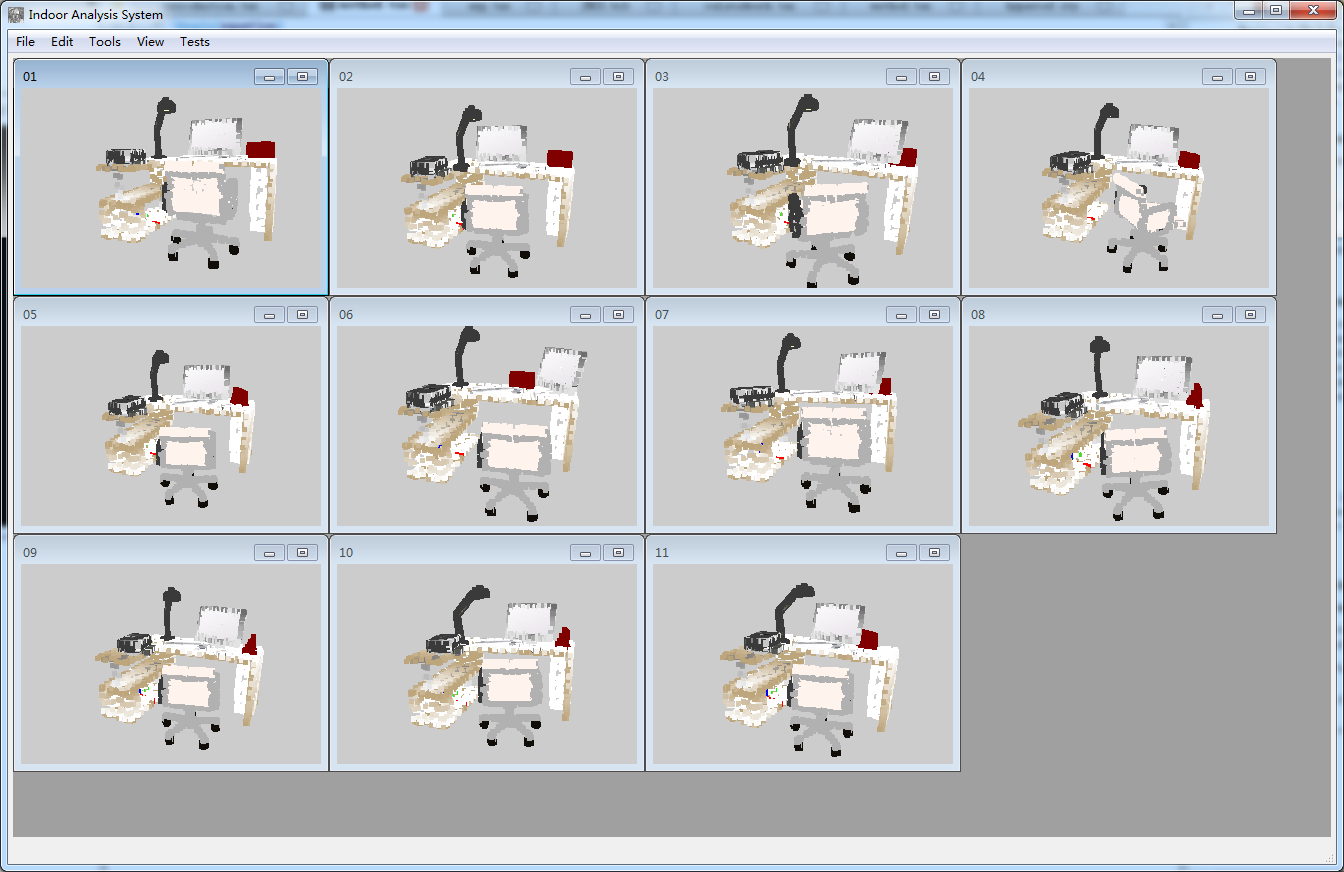
\includegraphics[width=.3\linewidth]{images/interact01.png}
	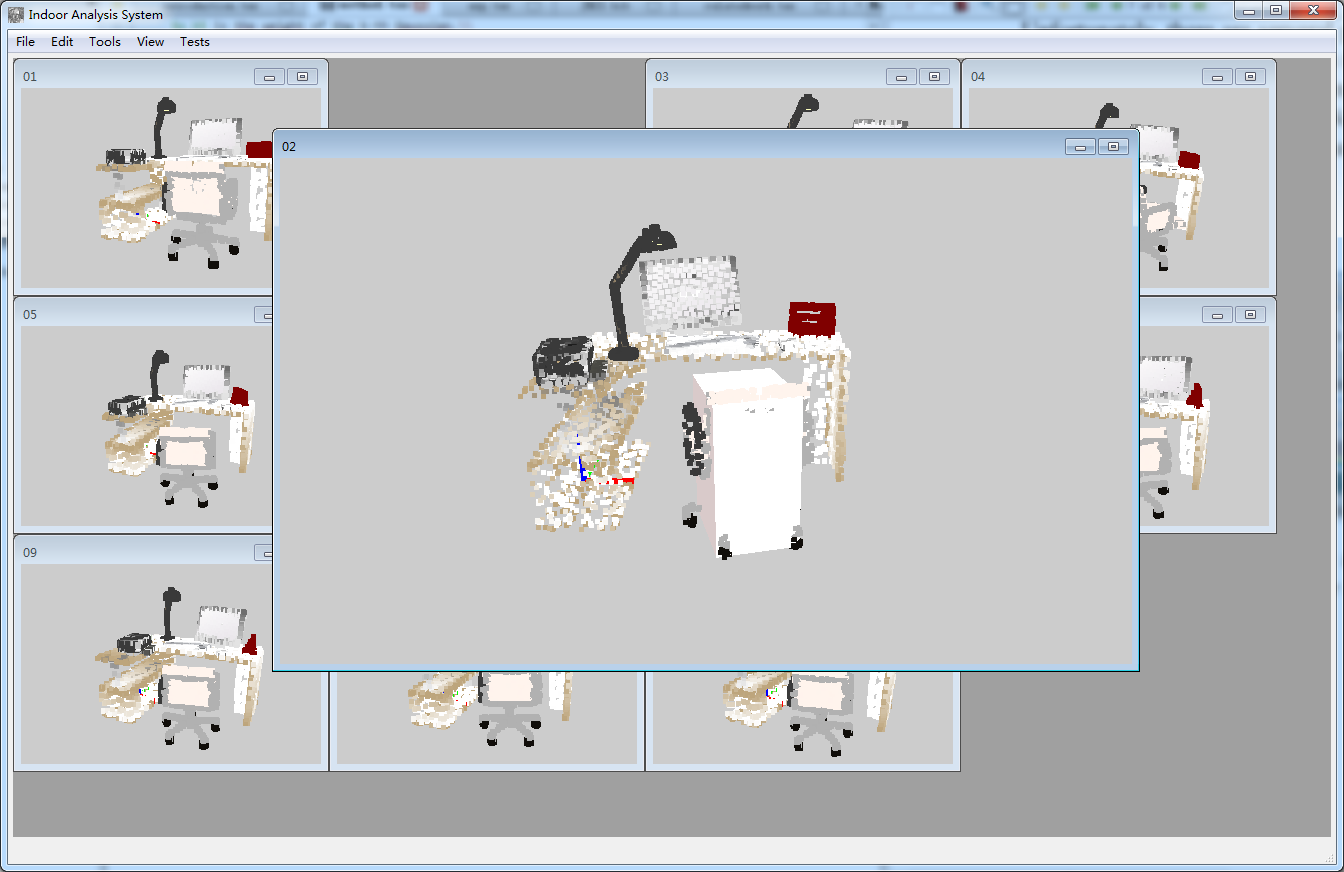
\includegraphics[width=.3\linewidth]{images/interact02.png}
	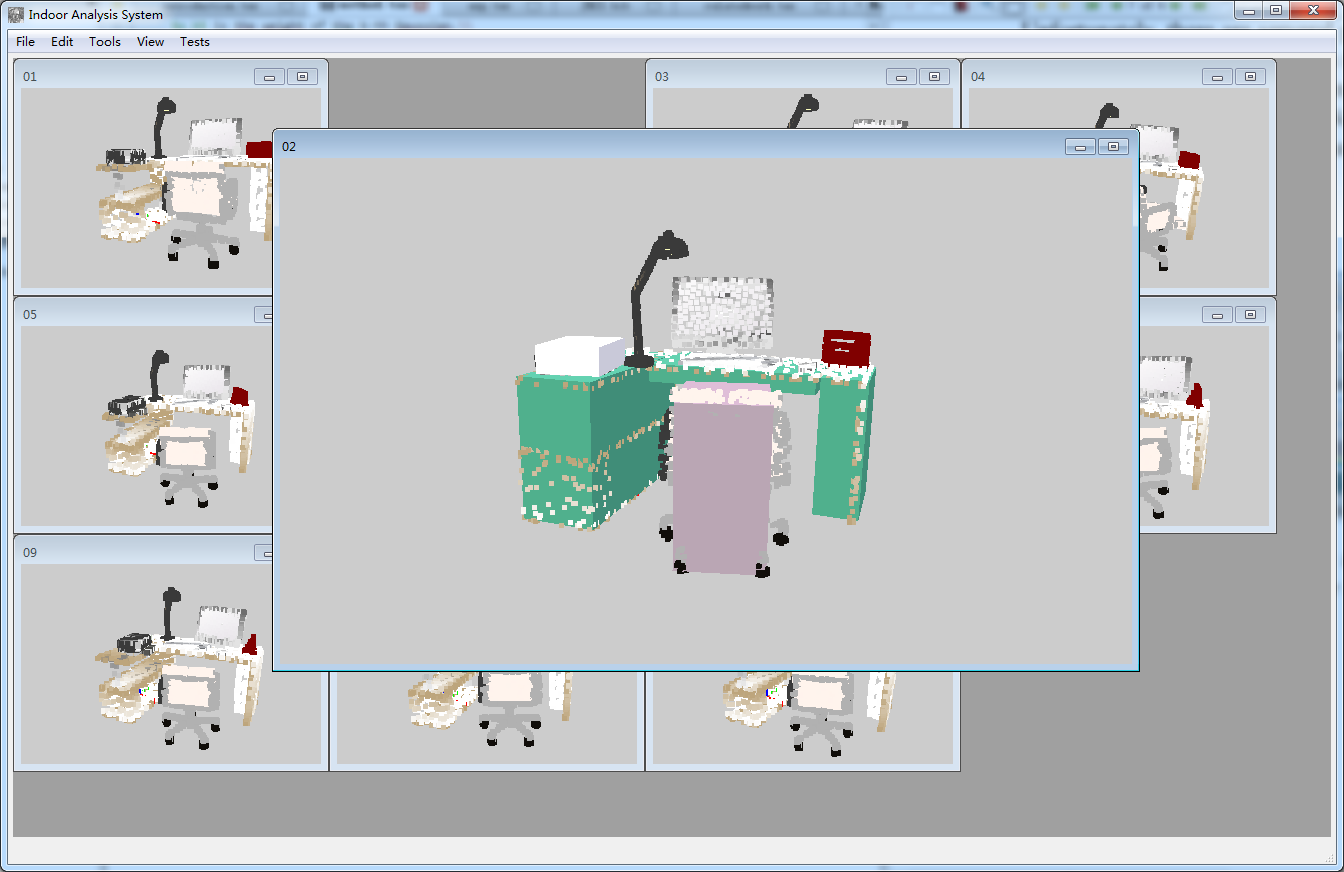
\includegraphics[width=.3\linewidth]{images/interact03.png}
	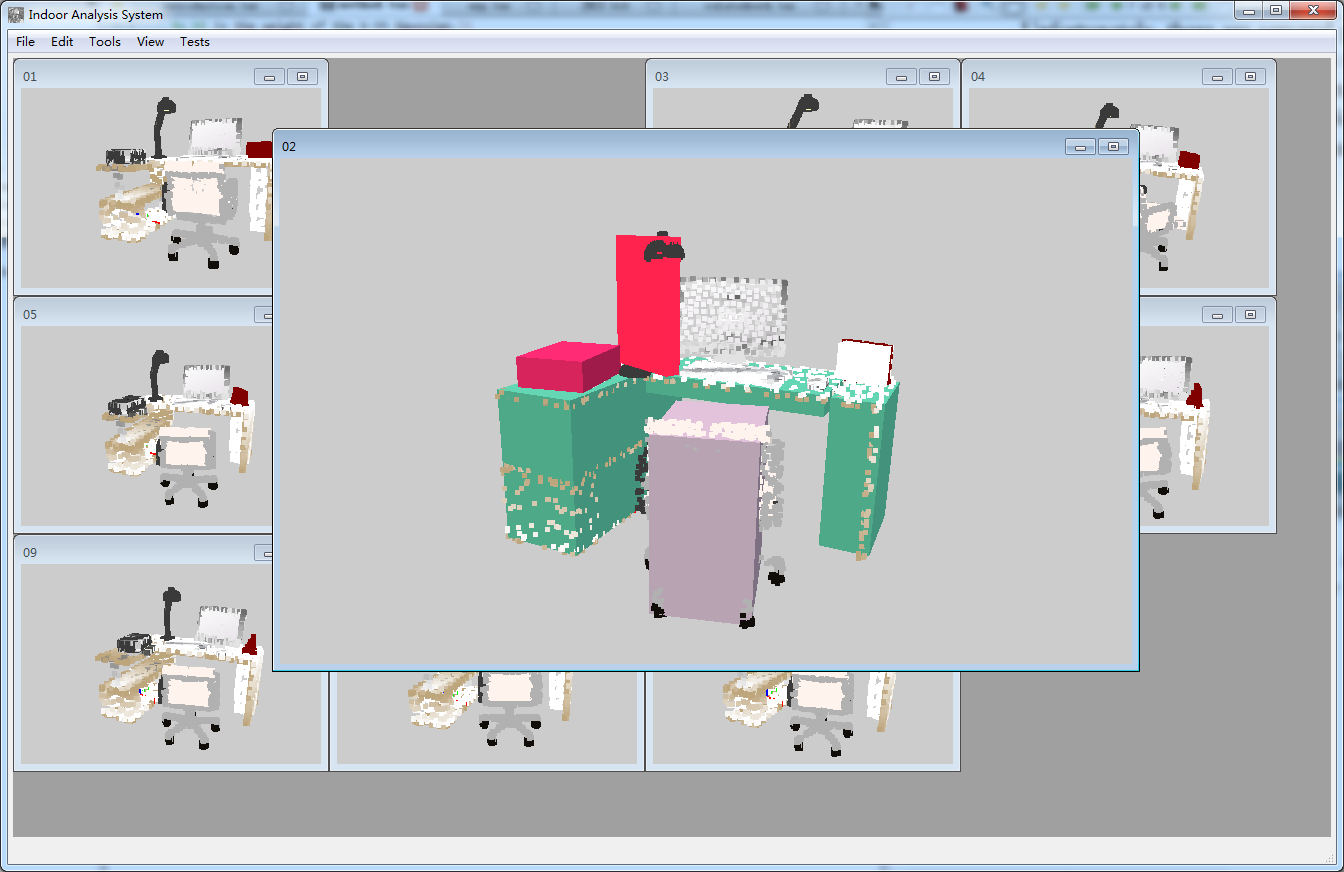
\includegraphics[width=.3\linewidth]{images/interact04.png}
	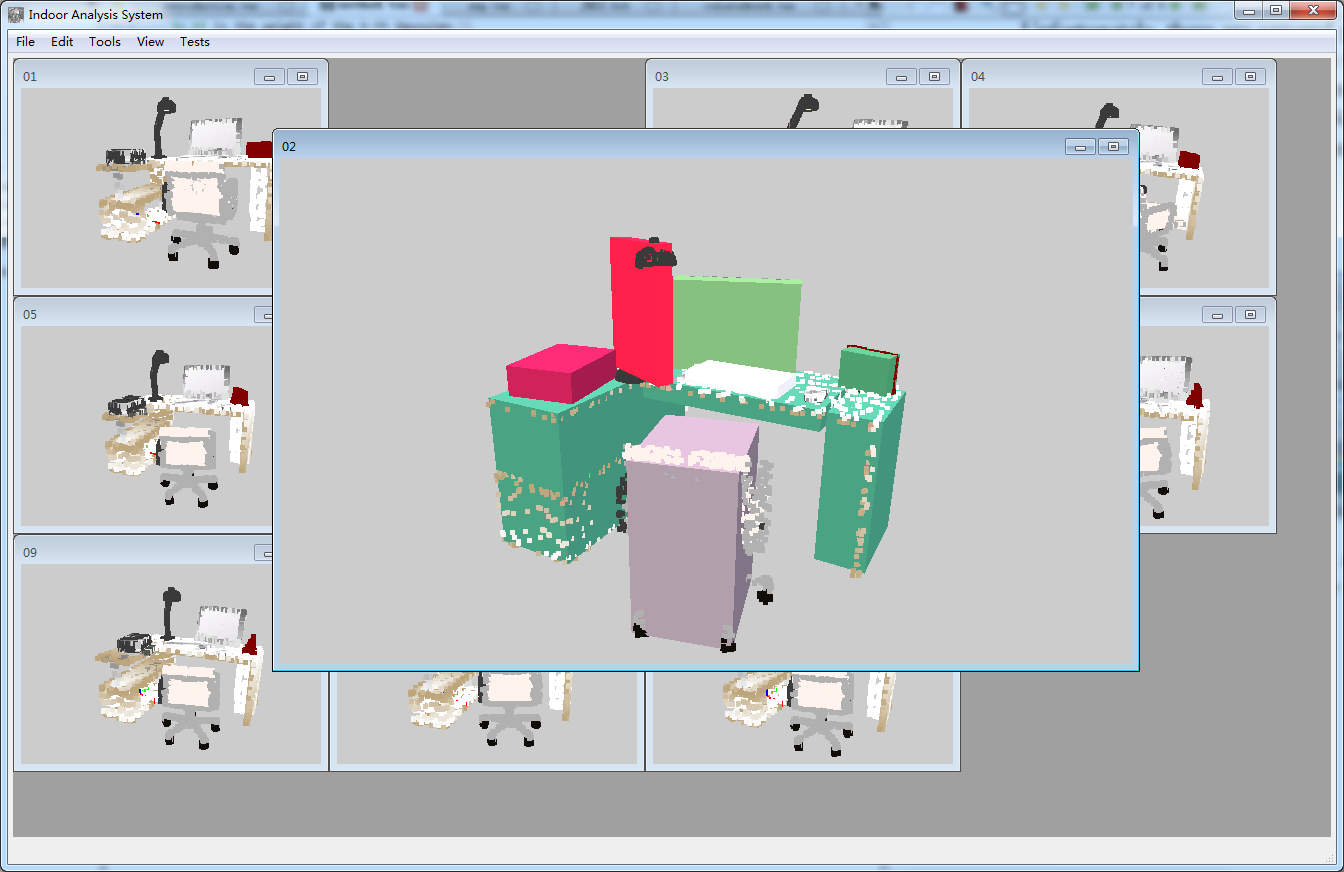
\includegraphics[width=.3\linewidth]{images/interact05.png}
	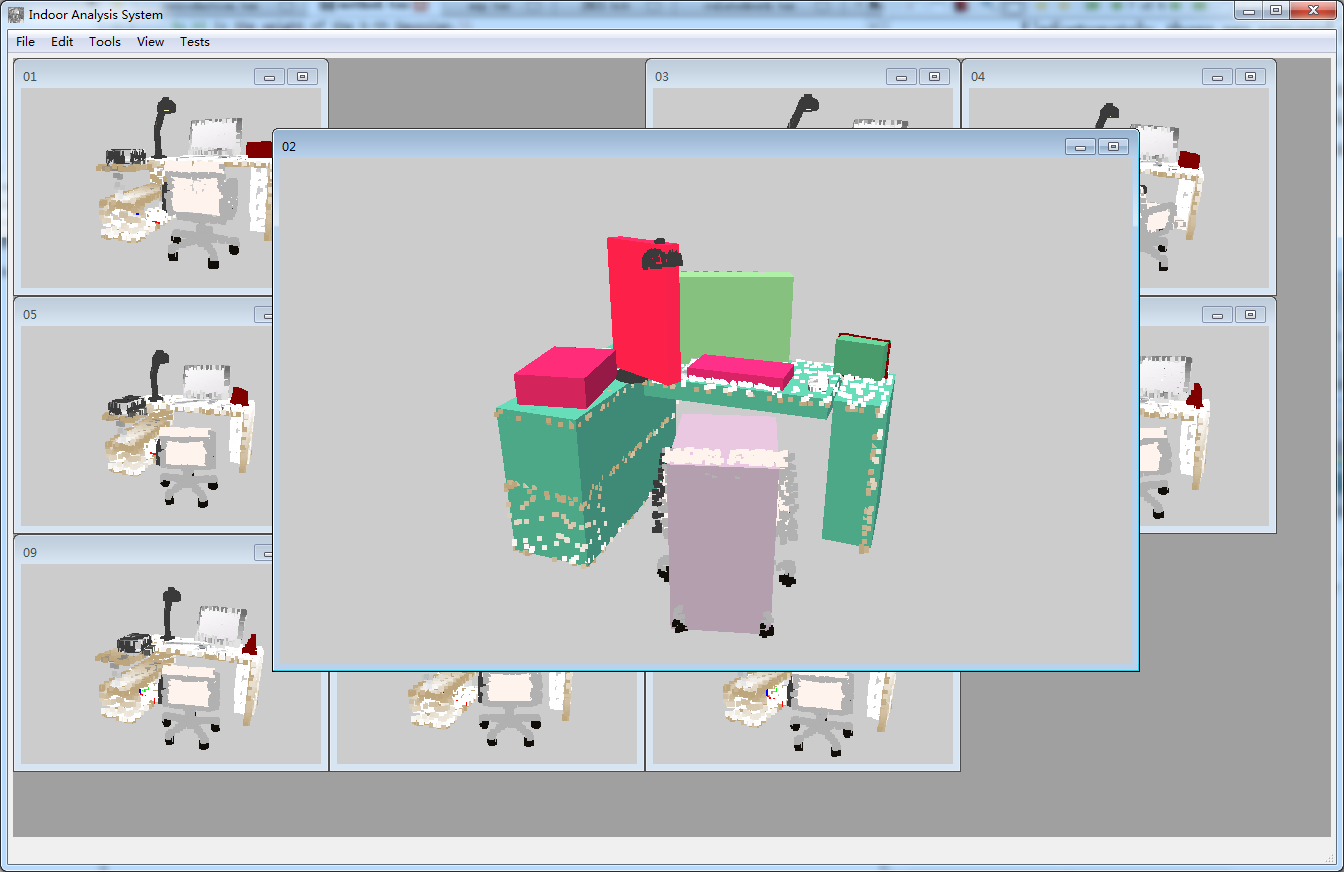
\includegraphics[width=.3\linewidth]{images/interact06.png}
	\caption{\label{fig:interact}
		From the first to the nineth, the nine images show the procedure of interaction:
		the user pick one point set and place boxes in it to indicate the layout for this point set. The box in white is the box currently under editing. The boxes in other colors are boxes placed to represent object layouts. One color represent one object. The interaction allows multiple boxes to represent same object.(e.g. the desk is represented by three boxes in same color)}
\end{figure}
These two paremeters are difficult to be initialized without semantic prior, but with the input of the users we can naturally initialize the $N$ as the number of different color label and the ${K_n}$ as 
\begin{equation}
\label{equ:K_n}
K_n=\frac{V_n}{\sum V_n}K_{all}
\end{equation}
in which the $V_n$ represent the total volume of the boxes in the $n^{th}$ color and the $K_{all}$ is initialized as $K_{all}=\frac{median(I_m)}{2}$ and $\{I_m\}$ are point numbers of $M$ input point sets. This is an emperical choice borrowed from \cite{Evangelidis2014}.\\
The expectation maximizaton framework is easily converged to a local optimal. To cope with this problem we further use this layout (boxes) from interaction as a soft constraint to guide the optimization and constrain the shape of generated object model. Such constraint is enforced by simply altering the posterior probability $\alpha_{mik}$ as\\
\begin{equation}
\label{equ:alteralpha}
\alpha_{mik}^*=\frac{\alpha_{mik}\beta_{mik}}{\sum_{i,k}\alpha_{mik}\beta_{mik}}
\end{equation}
where the $\beta_{mik}$ is the prior probability according to the boxes. It is defined as:\\
\begin{equation}
\beta_{mik}=\left\{
\begin{array}{rcl}
1& &\pmb v_{mi} \in B_n\\
\exp(-\frac{\min_{\pmb v_{mj}}|| \pmb v_{mi} - \pmb v_{mj} ||_2^2  )}{L})& &\pmb v_{mi} \notin B_n~and~\pmb v_{mj} \in B_n\\
\end{array} \right.
\end{equation}
where the $B_n$ is a point set that is enclosed by the boxes used to represent the layout of $n^{th}$ object. The $k^{th}$ Gaussian model is predefined to be one of the Gaussians used to represent $n^{th}$ object. $\min_{v_{mj}}|| v_{mi} - v_{mj} ||_2^2$ is actually the squared euclidean distance from point $v_{mi}$ to the point set $B_n$, as we define the distance from a point to a point set as the minimum distance from the point to any point inside the point set. $L$ here is a constant number with $L=2r^2$, and $r$ is the meadian of the radius of input point sets. The radius of a input point set is half of length of diagnonal line of its axis aligned bounding box.   
\begin{figure}[htb]
	\centering
	\includegraphics[width=\linewidth]{images/localoptimal/localoptimal}
	\caption{\label{fig:localoptimal}This figure shows an example result when converges to a local optimal. (a) is the result of segmentation of this local optimal. (b) is the final centroids of latent model. It shows that from top to down the 2nd and 3rd object model both include part of the table and part of the chair.}
\end{figure}
This alteration on posterior probability is only done with the probability related to the $m^{th}$ point set that have the mannual input layout (the boxes) in it. This alteration can help prevent the optimization from converging to a local optimal as in Figure~\ref{fig:localoptimal}. The result from the Figure~\ref{fig:localoptimal} have the same input and initialization with the result from Figure~\ref{fig:teaser}, but it doesn't use the posterior alteration as a soft constraint.

